\documentclass{beamer}

\usepackage[utf8]{inputenc}
\usepackage[danish]{babel}
\graphicspath{{../imgs/}}

\usetheme{Ilmenau}
\usecolortheme{beaver}
\uselanguage{Danish}
\languagepath{Danish}
\usepackage{xcolor}

\newcommand{\unit}[1]{\ensuremath{\:\text{#1}}}
\newcommand{\pro}{\ensuremath{\unit{\%{}}}}
\graphicspath{{../imgs/}}

\expandafter\def\expandafter\insertshorttitle\expandafter{%
  \insertshorttitle\hfill%
  \insertframenumber\,/\,\inserttotalframenumber}

\title{DaLUKE}
\subtitle{
    Den Dansktalende Sprogmodel MED VIDEN
}
\author[Søren Holm, Asger Schultz]{Søren Winkel Holm, Asger Laurits Schultz}
\institute[DTU]{Danmarks Tekniske Universitet}
\date{7. juli 2021}

\begin{document}

\begin{frame}
    \titlepage
\end{frame}

%Kom hurtigt til resultater
%Relativt få slides
%Vis arbejde
%Understøt med figurer
%Evt demonstrerer med karaktereksempel
%Kort om anvendelse - meget efterspurgt i industrien
%Kom hurtigt frem til resultater
%Hav repræsentationen med

% Asger: Hvad er problemet? og Hvordan gik det?
% Søren: Hvordan vil vi løse det? og Hvad har vi lært?

\begin{frame}
    \frametitle{Fremlæggelsen}
    \footnotesize
    \tableofcontents
\end{frame}

\section{Hvad er problemet?}
\begin{frame}
    % 1
    \frametitle{Mangel på viden og lavresourcesprog}
    \begin{itemize}
        \item På trods af grammatisk korrekt og idiomatisk tekst ved modeller ikke, hvad de taler om\footnotemark
        \item Det forsøges løst med viden
        \item I lavresourcesprog fungerer det også som en udvidelse af datasæt
        \item Fx er den engelske Wikipedia $ \sim 40 $ gange større end den danske
    \end{itemize}
    \footnotetext{\url{https://www.technologyreview.com/2020/08/22/1007539/gpt3-openai-language-generator-artificial-intelligence-ai-opinion}}
\end{frame}

\begin{frame}
    % 1
    \frametitle{Navngiven entitetsgenkendelse (NER)}
    \begin{itemize}
        \item Mål: Finde strengt definerede verdslige objekter i et dokument
        \item Praktiske anvendelser som informationssøgning, spørgsmålsbesvarelse og anonymisering
    \end{itemize}
    \begin{example}
        "Cæsar marcherede mod Rom og trodsede dermed det romerske senat."\\
        "Cæsar": person\\
        "Rom": sted\\
        "det romerske senat": organisation
    \end{example}
\end{frame}

\section{Hvordan vil vi løse det?}
\begin{frame}
    % 2
    \frametitle{Hvad gør Lukas anderledes?}
\end{frame}

\begin{frame}
    % 3
    \frametitle{Prætræning af DaLUKE}
\end{frame}

\section{Hvordan gik det?}
\begin{frame}
    % 3
    \frametitle{NER på dansk}
    Primært datasæt: \emph{DaNE} med 5.512 annoterede sætninger, heraf $ \sim 10\pro $ til validering og $ \sim 10\pro $ til test
    \begin{columns}
        \column{0.45\textwidth}
        \begin{itemize}
            \item Fire kategorier: LOC, PER, ORG og MISC
            \item Hovedmodel: Prætrænet i 150 epoker og fine-tunet i 15.
            Opnår 82,9\pro\ med MISC og 85,2 uden -- andenplads på DaNLP's liste
        \end{itemize}
        \column{0.55\textwidth}
        \begin{figure}[H]
            \centering
            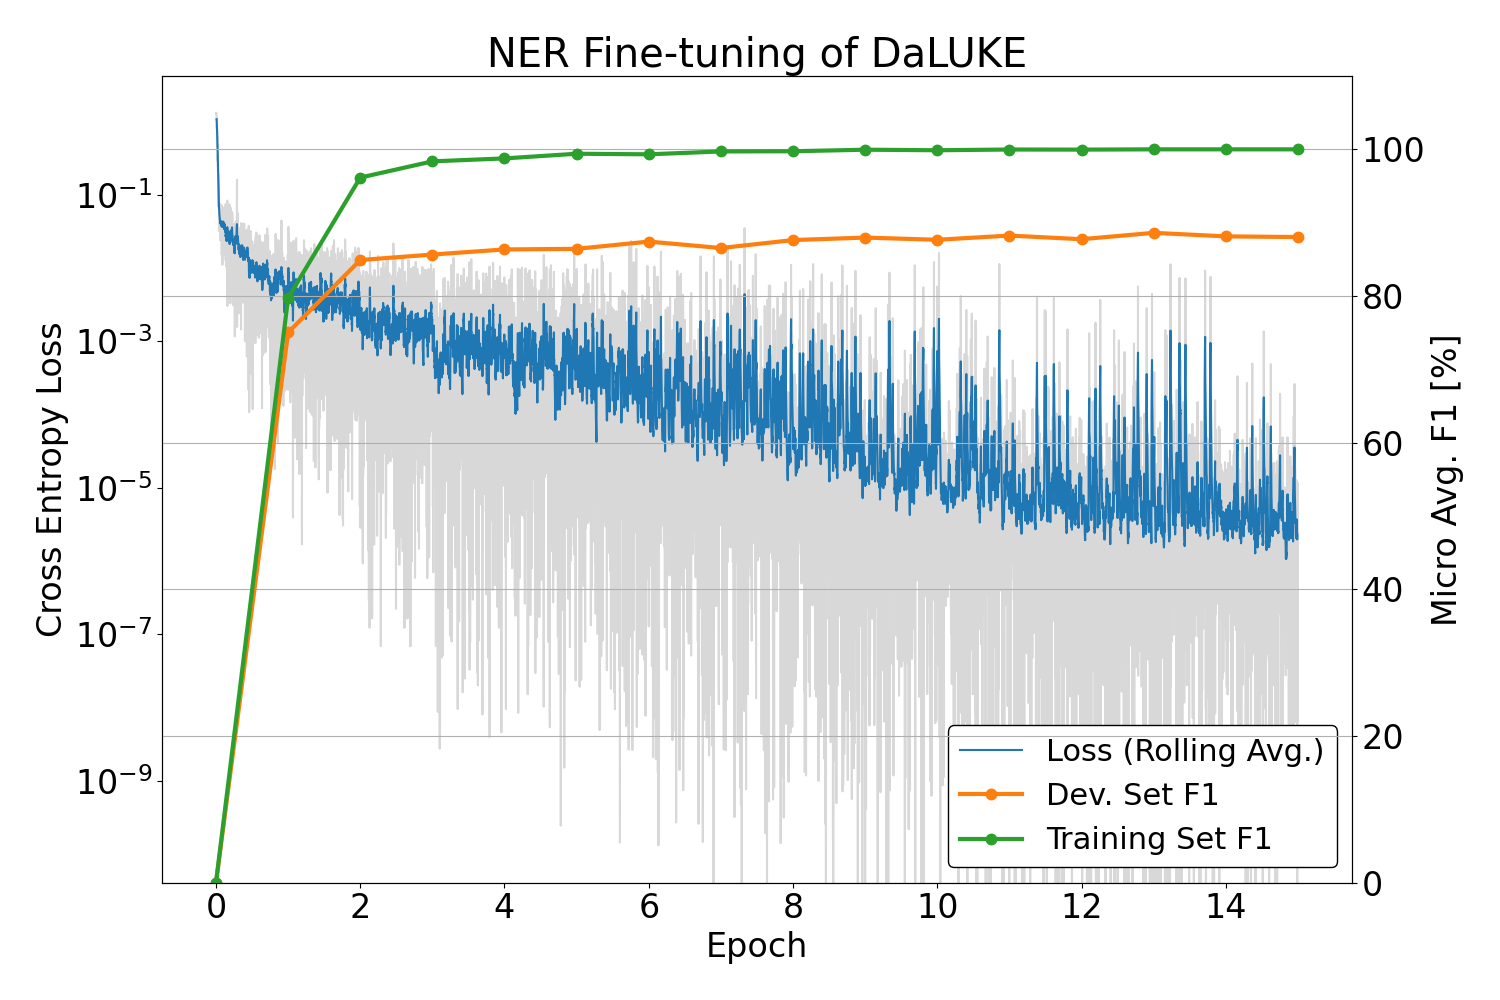
\includegraphics[width=\textwidth]{loss-fine}
        \end{figure}
    \end{columns}
\end{frame}

\begin{frame}
    % 3
    \frametitle{Entitetsbevidst selvopmærksomhed}
    \begin{itemize}
        \item Transformerudvidelse, der modellerer entitets-entitets- og ord-entitets-forhold direkte
        \item LUKE bruger ikke entitetsbevidst selvopmærksomhed i prætræningen, men DaLUKE gør
        \item Bedre resultater dog påvist i diverse fine-tuningsopgaver
        \item Uden brug i prætræning falder fine-tuningsresultater med 2,8 procentpoint
    \end{itemize}
\end{frame}

\begin{frame}
    % 3
    \frametitle{Transferlæring}
    \begin{columns}
        \column{0.4\textwidth}
        \begin{itemize}
            \item Hvad hvis man ikke initialiserede fra da-BERT?
            \item Langt bedre præcision i prætræning - tyder på overfitting
            \item Fine-tuning ligger 11,4 procentpoint under baseline
            \item Transferlæring virker stabiliserende og regulariserende
        \end{itemize}
        \column{0.6\textwidth}
        \begin{figure}[H]
            \centering
            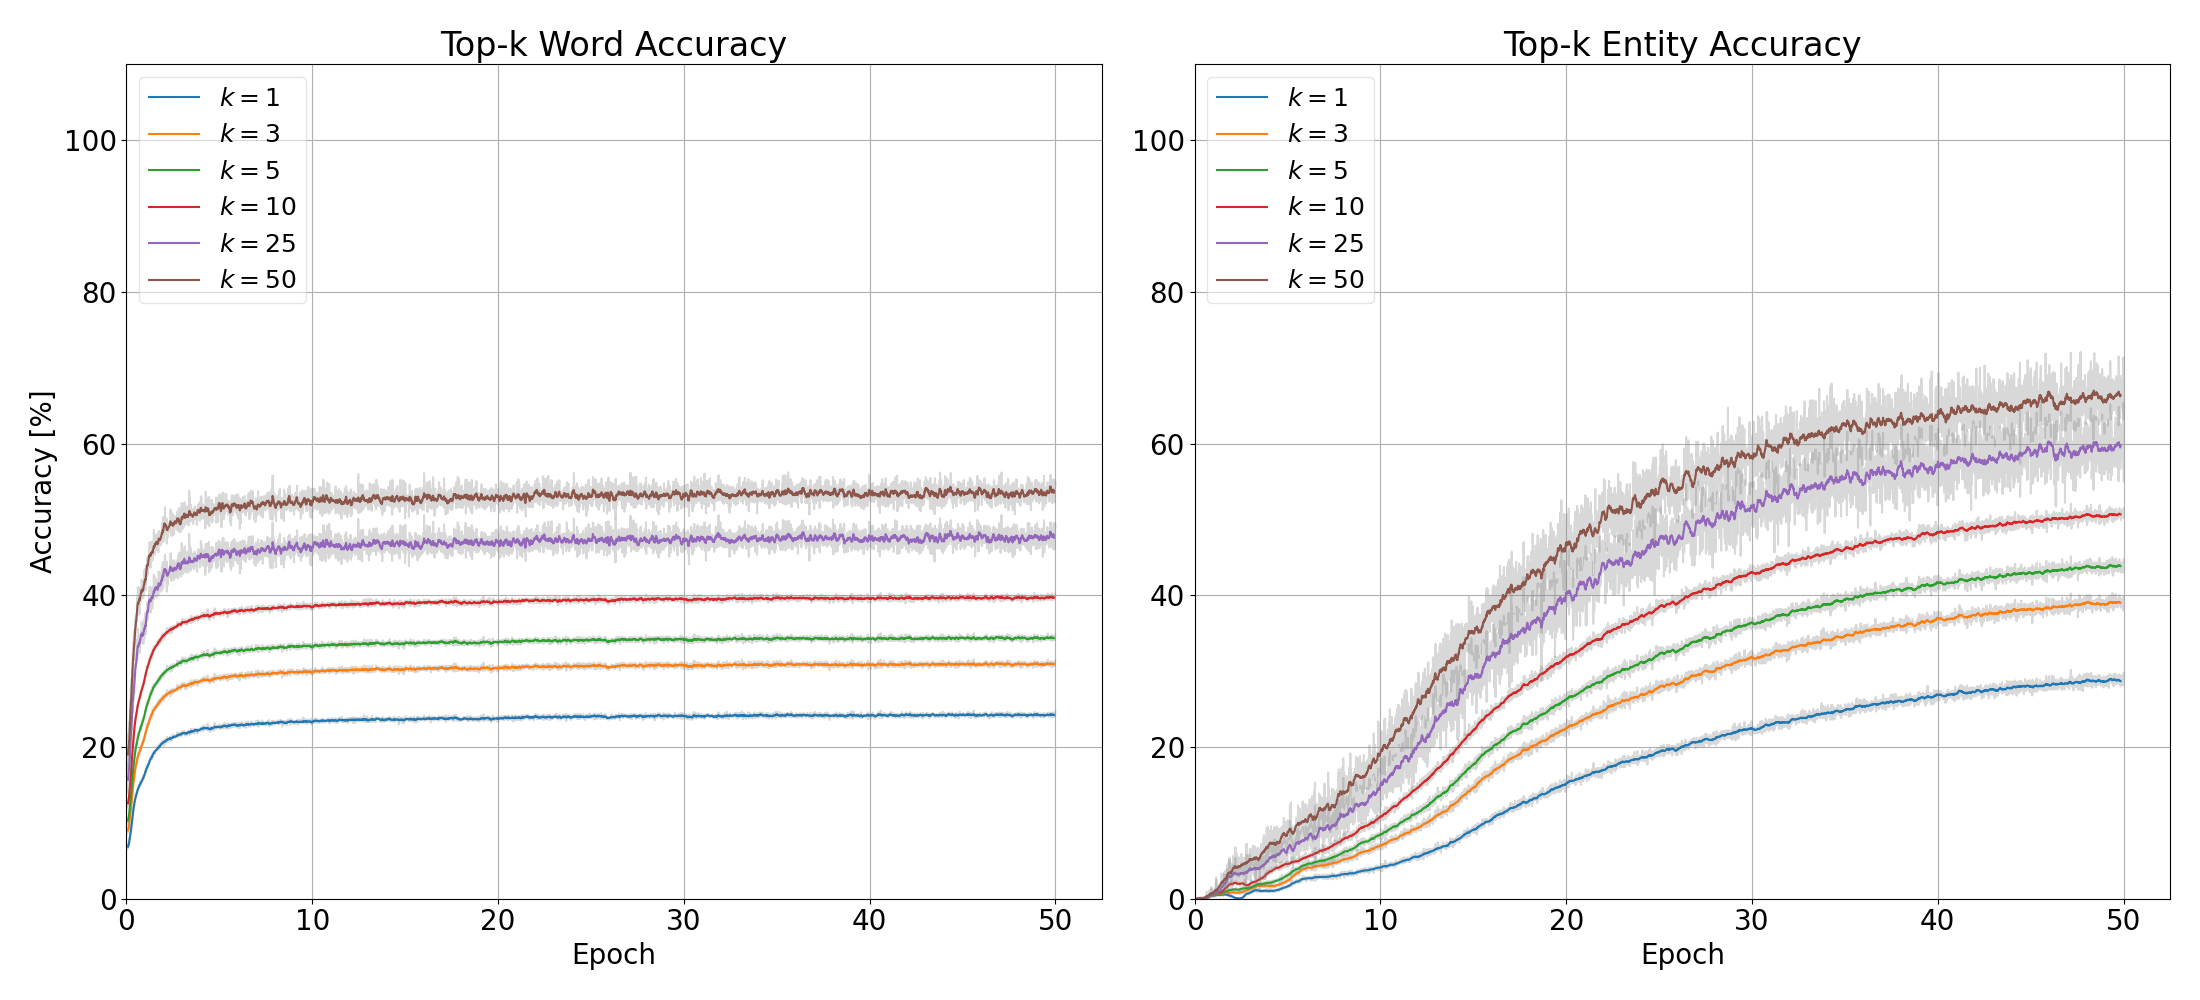
\includegraphics[width=.85\textwidth]{baseline-acc}
            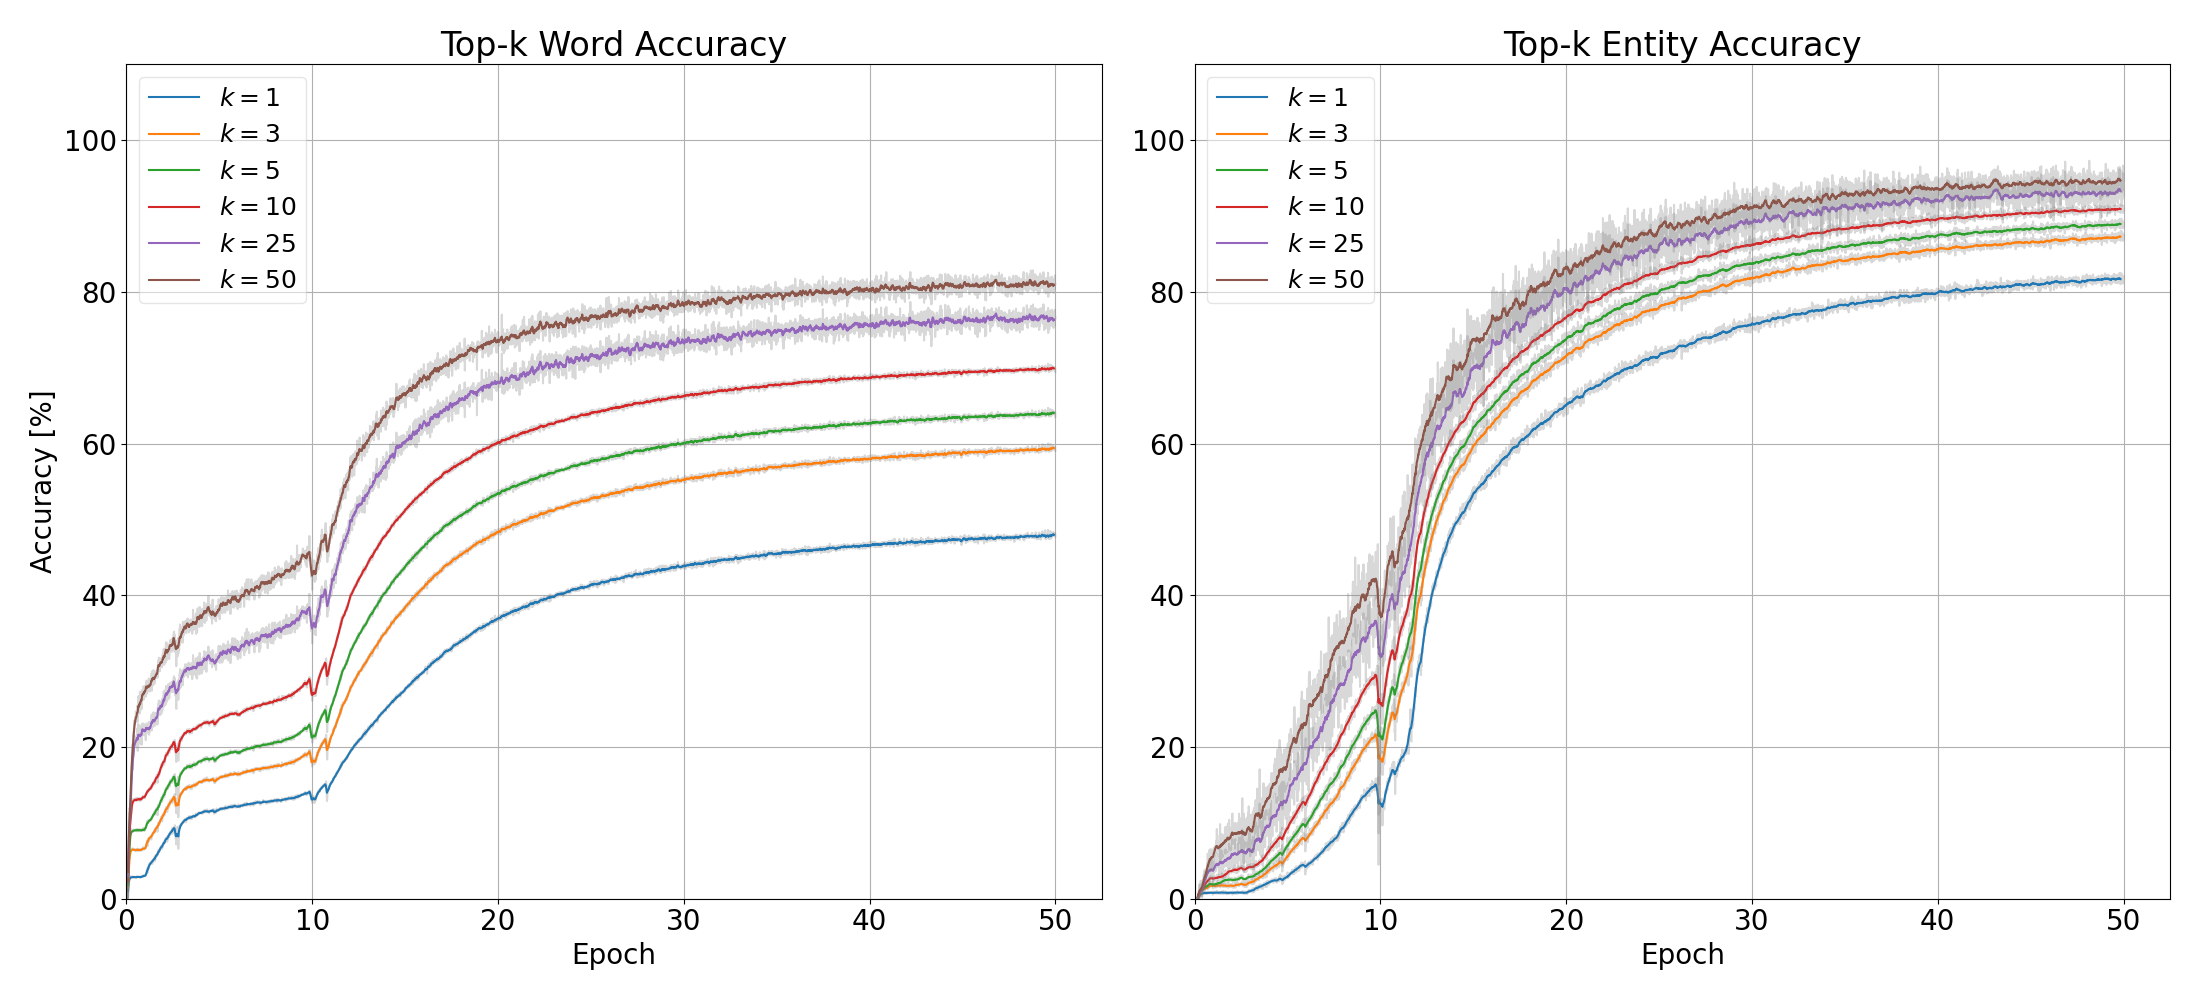
\includegraphics[width=.85\textwidth]{nobert-acc}
            \caption{Øverst: Baseline. Nederst: Ingen transferlæring}
        \end{figure}\noindent
    \end{columns}
\end{frame}

\begin{frame}
    % 2
    \frametitle{Datasætmodifikationer}
    \begin{itemize}
        \item Datasæt udvides med ekstra entiteter automatisk: $ 47\pro $ flere
        \item Uden dem fås 0,6 procentpoint højere; dog lille forskel ift. varians
        \item I LUKE beskæres entitetsordforrådet til de mest brugte. Hvilken effekt har det i DaLUKE?
        \item 0,2 procentpoint lavere med færre entiteter
    \end{itemize}
    \begin{example}
        "Arkæologi er studiet af tidligere tiders {\color{red}menneske}lige {\color{red}aktivitet}, primært gennem studiet af {\color<2>{blue}menneske}ts materielle levn. Langt det meste af al {\color<2>{blue}menneske}lig {\color{red}aktivitet} foregik, før vi lærte at skrive, så {\color<2>{blue}arkæologi} er den vigtigste metode til at studere ældre {\color<2>{blue}menneske}skabte samfund."
    \end{example}
\end{frame}

\section{Hvad har vi lært?}

\begin{frame}
    % 2
    \frametitle{NER er tilfældigt}
    % Lille sample
    % RNG
    % Krydsvalidering
\end{frame}

\begin{frame}
    % 3
    \frametitle{Repræsentationer}
\end{frame}

\begin{frame}
    % 3
    \frametitle{Forudsigelseseksempler}
\end{frame}

\begin{frame}
    % 1
    \frametitle{Afslutning med maskot}
\end{frame}

\end{document}
